\documentclass[10pt,a4paper]{report}
\usepackage[latin1]{inputenc}
\usepackage{amsmath}
\usepackage{amsfonts}
\usepackage{amssymb}
\usepackage{graphicx}
\usepackage[danish]{babel}
\usepackage{hyperref}

\title{Webintelligence - Mini Project 3}
\author{Lars Andersen, Mathias Winde Pedersen \& S�ren Skibsted Als}
\begin{document}
\maketitle

\section*{Part 1 - Data Manipulation}
The first part of the project is to load data.
The data consists of two parts, training data and probe data.
A subset of this is loaded, as if you were to load all of it, the loading and later training would take too much time.

One thing you have to be careful about, though, is that the probe data is part of the training data.
This is bad as you would then get to train on the test set.
In order to prevent this, we remove the probe part from the training set, and instead store its actual ratings in the probe set, to be used for later testing of the algorithm.

This transformation of the data is performed once, such that you do not need to perform this conversion each time you test your program.

\section*{Part 2 - Learning}

\subsection*{Recommender Systems}
Two sorts of recommender systems have been talked about during the lectures:
\begin{itemize}
   \item Content-based filtering
   \item Collaborative filtering
\end{itemize}

The content-based filtering has to do with predictions based on the content, that is if you have reviews, geographics, gender, and other kinds of such information.
Collaborative filtering is to predict based on other peoples ratings, where people more similar to you has a greater influence.
For the netflix dataset, no real content is provided other than the title, however, a vast amount of user movie pair ratings are provided.
This leads to the obvious choice of using collaborative filtering.

In a broader setting, where you have access to the content and other users ratings, a mix of the two is beneficial.

\subsection*{Matrix Factorization}
In the area of collaborative filtering, several approaches can be taken.
These include item-based, user-based and latent factor models(Matrix Factorization).
The matrix factorization model is for this dataset preferred. This is due to the dataset being very large.
As the dataset is very large, we trade a complex offline model for a fast online prediction. Additionally, if you were to use some of the other approaches, as the dataset is so large, it cannot fit in main memory, whereas the matrix factorization approach is more scalable, such as the netflix dataset with about 17k movies and 240k users.
How the approach then works is to approachimate the single value decomposition matrix (SVD).
Libraries exist to calculate this, however, as such a computation can be quite heavy, another approach is used called Funk-SVD.

\subsection*{Funk-SVD}
The idea behind the algorithm is to tackle the problem that the user-movie matrix is very large but very sparse.
That is mainly the result of each user only watching a small fraction of the entire movie set.
In order to utilise this to instead work on smaller matrices, a "squeezing" of the matrix is performed, such that we instead work on K factors/topics.

\begin{figure}[h]
	\centering
	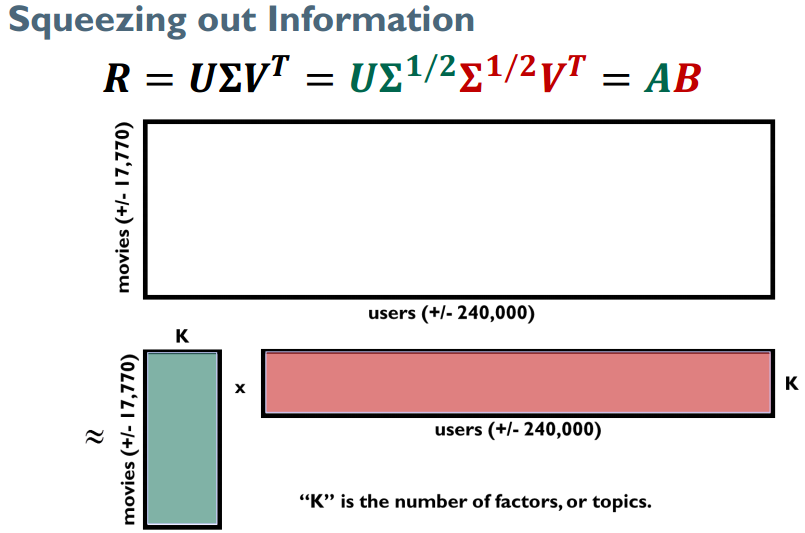
\includegraphics[scale=0.3]{slidesqueeze}
	\caption{Matrix squeezing, taken from the slides.}\label{matrix:squeeze}
\end{figure}

An illustration of the theory for this can be seen in Figure \ref{matrix:squeeze}.
These two smaller matrices can then be interpreted in different ways.
Each row in the movie-matrix $U$ then represents $k$ genres, and the given movie's values for each genre, such that movies similar have similar values for the different genres.
If you look at the user-matrix $V$ each column corresponds to the values for each movie genre of a user, such that users with similar tastes in movies will have similar values for their columns. These rows/columns could also be interpreted as movie/user communities, but we take the first interpretation approach.

The matrix we then want to calculate is as follows:
$$\hat{R}_{mu} = \sum_{k=1}^{K}{A_{mk}*B_{ku}}$$

We then want to produce $A$ and $B$ to be able to reproduce the observed ratings as best as possible.
To do this we want to minimize the squared error, this is involved with what $K$ we choose, and is touched upon in the scoring section.
The trick then comes into play.
We train and minimize the error for the observed ratings only, and as of such ignores the non rated movie-user pairs.
Then when you multiply $A$ and $B$ then non non-rated movie user pairs will have ratings calculated, these ratings then serves as our prediction!
In other words, the non-rated movie-user pairs is then learnt from the observed ratings of similar users/movies.


In order to minimize the error, we use stochastic gradient descent to approximate $A$ and $B$. The reason a stochastic gradient descent and not a usual gradient descent is used, is due to the fact that the regular gradient descent would not scale well with the large netflix dataset.

How this stochastic gradient descent is used can be seen in Figure \ref{stochasticgradientlabel}.
\begin{figure}[h]
	\centering
	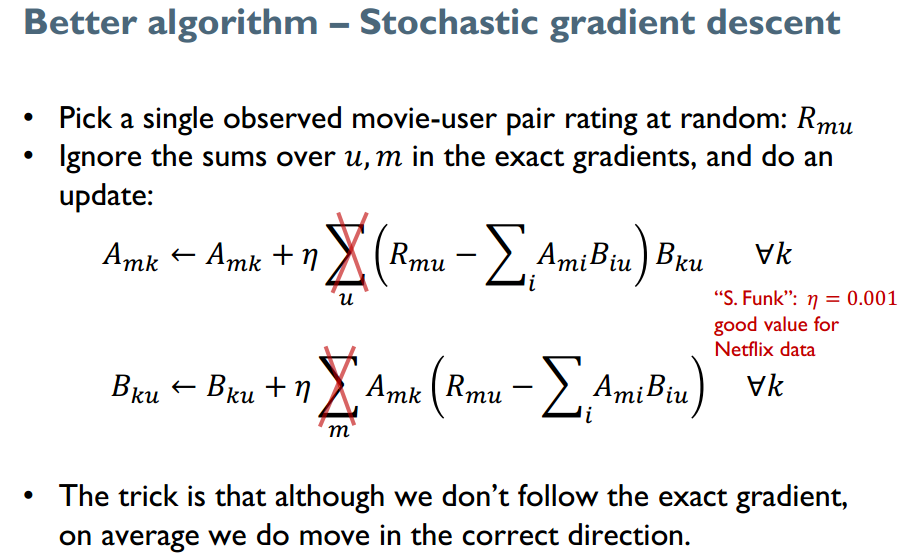
\includegraphics[scale=0.3]{stochasticgradient}
	\caption{Stochastic Gradient Descent}\label{stochasticgradientlabel}
\end{figure}
One problem with this is that the stochastic gradient descent will not converge to the minimum, but instead "dingle" around it.
This can then be resolved by using a weighted decay.

Apart from this some preprocessing steps of the ratings needs to be performed and is discussed hereafter.
\subsection*{Preprocessing Step}
Before we use the stochastic gradient descent to approximate $A$ and $B$ we need to perform some preprocessing on $R_{mu}$.
What we want to do is subtract the user and movie means and add the overall mean.
The reason we want to substract the user mean and movie mean is to adjust the ratings to be around zero. However, as you subtract two times for each entry, you have adjust with the overall mean, which is why this is added.
We did this preprocessing step and made sure that the overall sum of the preprocessed entries and found it was very close to zero ($10^{-8}$) which was sufficient, and ensured that the preprocessing did not "skew" the data too much. 
The reason it was not entirely zero is blamed on floating point numbers to be inaccurate.
So the algorithm for this preprocessing step then is as follows:
$$R_{mu} = R_{mu} - \frac{1}{U_m}*\sum_{s}{R_{ms}} - \frac{1}{M_u}*\sum_{r}{R_{ru}} + \frac{1}{N} * \sum_{s}{\sum_{r}{R_{sr}}}$$

\begin{itemize}
	\item[text]
	\item[text]
	\item[text]
\end{itemize}
It is then important after the stochastic gradient descent to add these values that you removed.
And thus finally you do the following calculation.

$$\hat{R_{mu}} = \hat{R_{mu}} + \frac{1}{U_m}*\sum_{s}{R_{ms}} + \frac{1}{M_u}*\sum_{r}{R_{ru}} - \frac{1}{N} * \sum_{s}{\sum_{r}{R_{sr}}}$$
\section*{Part 3 - Scoring}

\subsection*{Evaluation of RMSE}

\subsection*{Evaluation of k}

\end{document}